%%%%%%%%%%%%%%%%%%%%%%%%%%%%%%%%%%%%%%%%%%%%%%%%%%%%%%%%%%%%%%%%%%%%%%%%%%%
% % Plantilla para un artculo en LaTeX en espaol.  %
%%%%%%%%%%%%%%%%%%%%%%%%%%%%%%%%%%%%%%%%%%%%%%%%%%%%%%%%%%%%%%%%%%%%%%%%%%%

\documentclass[12pt,twoside,onecolumn]{article}

% Esto es para poder escribir acentos directamente:
%\usepackage[latin1]{inputenc} 
\usepackage[utf8]{inputenc}
\usepackage{makeidx} \usepackage{multirow} \usepackage{titlesec}
\usepackage{sectsty} \usepackage{fncychap}

%\usepackage{natbib}

\renewcommand{\thesection}{}
\renewcommand{\thesubsection}{\arabic{subsection}}
% Esto es para que el LaTeX sepa que el texto est en espaol: 
\usepackage[spanish]{babel}
\usepackage[right=3cm,left=3cm,top=2.5cm,bottom=2.5cm,headsep=1cm,footskip=2cm]{geometry}
\usepackage{graphicx}
% Paquetes de la AMS: 
\usepackage{amsmath, amsthm, amsfonts}
\renewcommand{\thesection}{}
\renewcommand{\thesubsection}{\arabic{subsection}}
\usepackage{hyperref} 
%\pagestyle{headings} 
\pagestyle{myheadings}
\markboth{Documento de Dise\~no - Big Bobbin}{}

\begin{document} 
\setlength{\unitlength}{1 cm} %Especificar unidad de trabajo
\thispagestyle{empty}
%\begin{picture}(25,8)
%\includegraphics[width=14cm,height=9cm]{deu2.jpg}
%\end{picture}

\vspace*{-1in}
\begin{figure}[htb]
\begin{center}

\includegraphics[width=12cm]{./figures/deutlogo.png}
\end{center}
\end{figure}

\begin{center}
\textbf{
{\LARGE Departamento de Electr\'onica}}\\[1.25cm]
{\Large Documento de Dise\~no}\\[1.3cm]
{\LARGE \textbf{Operaci\'on Big Bobbin}}\\[2.5cm]
{\large Arturo Veras Olivos}\\[1cm]
Valparaiso - \today
\\[2cm]
{\texttt{\textit{Water eventually would be employed as a fuel and that the hydrogen and oxygen which constitute it would furnish an inexhaustible source of heat and light. Jules Verne}}}
\end{center}
 
%\newpage 
%\tableofcontents
%\listoffigures % to produce list of figures 
%\listoftables % to producelist of tables 
%\begin{abstract}
%   abstract-text
%\end{abstract}
\newpage 
\section{Alcance}
Este documento es un intento de entregar el fundamento teórico del funcionamiento de la electr\'olisis no convecional que pretende usar procesos no faradicos para la producci\'on eficiente de gas de kross para la combusti\'on o bien para almacenamiento. Esto para sentar las bases del dise\~no de un circuito de amplificaci\'on del Voltaje de actuaci\'on a una celda electrol\'itica.

\section{Introducción}
De acuerdo con la primera ley de faraday de la electrolisis~\cite{1954JChEd}, sabemos que \textit{La tasa de flujo de masa de gas es proporcional a la densidad de corriente}. En otras palabras: \textit{La masa de una sustancia producida en un electrodo durante la electrólisis es proporcional al número de moles de electrones (la cantidad de electricidad) transferido en ese electrodo}. Por lo tanto, el objetivo de un proceso de electrólisis de agua eficiente es alcanzar niveles más altos de corriente mientras se aplica el voltaje mínimo posible de la celda~\cite{kavehinvestiagtion}. La eficiencia de los generadores de hidrógeno modernos se mide por la energía consumida por unidad de volumen estándar de hidrógeno ($\frac{MJ}{m^3}$), suponiendo que la temperatura y la presión del hidrógeno estándar~\cite{h2vol}. Como dato, se han reportado eficiencias de trabajo para celdas alkalinas en 1996 en el rango de 50-60\% para pequeños electrolizadores y alrededor de 65-70\% en grandes plantas~\cite{eff}.\\

Existen investigaciones que plantean que el proceso de electrolisis no depende de energía. Según la teoría de Arrhenius, las moléculas dentro de una solución se disocian en iones y estos iones son recogidos en el electrodo\cite{dublin}, donde la energía de separación proviene del proceso de auto-ionización del agua. La mayoría de las investigaciones asumen que la energía calórica liberada en la combustión del resultado de la electrolisis procede de la combustión del hidrógeno pero cuando el gas utilizado es la combinación de hidrógeno y oxígeno producto de la electrolisis, la energía liberada tiene propiedades diferentesa las del hidrógeno. Sin embargo, se propone la hipótesis de que la energía dominante no proviene del gas hidrógeno, sino que proviene de grupos cargados de gas de agua, que activan coherente-mente la energía de punto cero.\cite{king2011water}



\section{Electrólisis del agua}
En la electrólisis, una corriente eléctrica DC se pasa a través de una sustancia conductora  (electrolito) con el fin producir una reacción no espontánea. Las semi-reacciones de interés es la descomposición del agua en hidrógeno y oxígeno~ presentadas en la ecuación~\eqref{reac:cat}~y~\eqref{reac:and} respectivamente; esta reacción es endotérmica, lo que requiere un aporte de energía. A todos los efectos practico, el agua pura no conduce la electricidad, por lo que se añade un electrolito para facilitar la reacción, usualmente se usa hidróxido de potasio. La figura~\ref{fig:electrolisis} se presenta la forma más simple de electrolisis del agua.

\begin{figure}
  \centering
   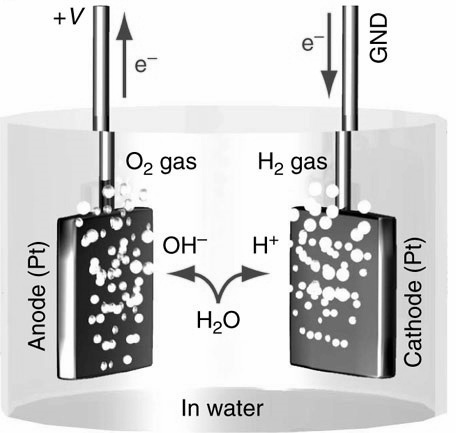
\includegraphics[width=0.5\textwidth]{figures/electrolisis}
  \caption{Electrolisis del agua con dos electrodos}
  \label{fig:electrolisis}
\end{figure}

\begin{equation} \label{reac:cat}
 Catodo: 2H^+ + 2e \rightarrow H_2
\end{equation}

\begin{equation} \label{reac:and}
 Anodo: 2OH^- \rightarrow \frac{1}{2} O_2 + H_2O + 2e
\end{equation}

\begin{equation}
 Total: H_2O \rightarrow H_2 +\frac{1}{2}O_2
 \end{equation}

El voltaje minimo necesario para que la reacción ocurra bajo presión y temperatura constante (1 bar, 25C) es
\begin{equation}
V_{min} = \frac{-\triangle G^0}{nF} 
\end{equation}
donde $-\triangle G^0$ es el cambio en la energía libre de Gibbs, $n$ es el numer de electrones transferidos y $F$ es la constante de Faraday. Para el caso ideal sin perdidas y de una celda de dos placas, $V_{min}=1.23 [V]$, con $-\triangle G^0 = 237.2 [\frac{kJ}{mol}]$. En la práctica, perdidas por la reacción y resistencias son inevitables resultando ineficiencias en el sistema, para cubrir estas perdidas se agrega energía adicional y se le conoce como el sobrepotencial. El resultado es un voltaje de operación $V_{op}$ y una corriente $I$ necesaria para llevar a cabo la reacción, de forma que,
\begin{equation}
V_{op} =  \frac{-\triangle G^0}{nF} + IR + \sum\eta
\end{equation}  
donde R es la resistencia ohmica de la celda que incluye el electrolito, los electrodos y resistencias externas; $\sum\eta$ es la suma de sobrepotenciales (sobrepotenciales de activación en los electrodos y el sobrepotencial por el transporte de masa de los gases que están lejos de la superficie de los electrodos). Finalmente la energía $E_{prod}$ para producir 1 mol de hidrógeno puede expresarse como
\begin{equation}
E_{prod}=V_{op}It
\end{equation}
donde t es el tiempo para producir 1 mol de hidrógeno~\cite{kim2006water}.

A medida que aumenta la densidad de corriente entre los electrodos, aumenta el sobrepontacial, lo que hace que se genere calor y da como resultado una pérdida de eficiencia. Pero a bajas densidades de corriente se produce muy poco gas para aplicaciones prácticas, por lo que se requiere un balance entre la densidad de corriente y los sobreponteciales~\cite{zeng2010recent}.

\section{Electrólisis No-Convencional / Gas de Kross}
Sobre la electrolisis no-convencional existen varías teorías que lo que puede estar sucediendo tanto a nivel atómico, molecular y eléctrico. Lo que si es claro es que existen anomalías del gas que está produciendo resultado de la electrolisis que no pueden ser explicadas a través de las propiedades del hidrógeno. A continuación se muestra algunos charlatanes, sus teorías y demostraciones.

\subsection{Andrija Pujari} Dice que inventó un dispositivo termodinamico para producir hidrógeno y oxígeno de agua ordinaria o agua de mar e inventó un nuevo metodo para descomponer la molécula de agua en hidrógeno y oxígeno a una eficiencia entre 80\% y 100\%. Su teoría se basa en manipular la geometría molecular angular del agua en que los pares de electrones sin compartir ejercen una repulsión que evita la formación de un tetraedro (109,5), por lo que los enlaces O-H forman entre sí un ángulo de 104,5~\cite{h2owiki}como muestra la figura~\ref{fig:h2o}. Para lograr esto, Andrija creó una cikim2006waterrcuito generador de ondas que coiciden con las complejas frecuencias de resonancia de la geomtría tetraedrica del agua~\cite{wiki:tetra}. Más detalles sobre la teoría y el dispositivo utilizado ver~\cite{puharich1983method}. Un resumen de su metodo a continuación.

\subsubsection{Genrador de señales}
Como lo describe Andrija, con el Componente I que está en la figura ~\ref{fig:comp1}, se generan  complejas formas de ondas a frecuencias que resuenen con las complejas frecuencias de los enlaces de la molecula de agua la que está altamente energizada en una geometría molecular tetraédrica con angulos de separación $109^o,28'$. Para esto, el Componente I automáticamente\footnote{No se explica a que se refiere con automaticamente por lo que no es posible detallar este proceso} sigue 7 estapas desde la estapa A a la F, de la tasa de reacción variando los parametros de frecuencia portadora de resonancia, forma de onda, corriente, voltaje e impedancia. El Componente 1 consite en un generador de frecuencia de audio (entre 20 Hz y 200 Hz) de amplitud modulada con una onda portadora (entre 200 Hz y 100,000 Hz). Particularmente en la etapa C es donde ocurre el fenómeno de máxima generación, acá se ajustan valores de voltaje y corriente a valores que causa que la onda cambie a un diente de cierra, ver~\ref{fig:sawtooth}, con frecuencia portadora $f_c=3980 Hz$, generando armónicos superiores en $f_{2c}=7960Hz$, $f_{3c}=15,920Hz$, $f_{4c}=31,840Hz$ y $f_{5c}=63,690Hz$. Esta forma de onda se dice que es necesaria para una eficiencia óptima para la electrólisis del agua, ya que se cree que cada una de estos armónicos resuena con cada uno de los cuatro ápices de la molécula de agua en su forma tetraédrica. 

\begin{figure}
  \centering
   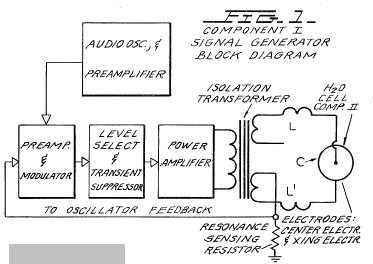
\includegraphics[width=0.7\textwidth]{figures/comp1}
  \caption{Componente 1 del sistema: Generador de señales}
  \label{fig:comp1}
\end{figure}

\begin{figure}
  \centering
   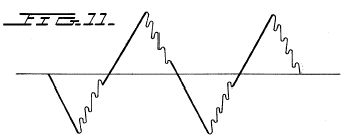
\includegraphics[width=0.5\textwidth]{figures/sawtooth}
  \caption{Componente 1 del sistema: Generador de señales}
  \label{fig:sawtooth}
\end{figure}

\subsubsection{Electrolisis}


%% Falta explicar en detalle la tecnoglía y teoría.
%% Mostrar funcionamiento de circuito

\begin{figure}
  \centering
   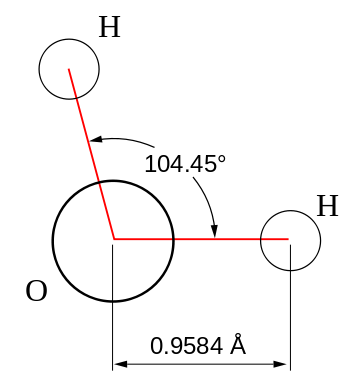
\includegraphics[width=0.3\textwidth]{figures/h2o}
  \caption{Geometría molecular angular del agua que forma un ángulo de 104,5}
  \label{fig:h2o}
\end{figure}

\subsection{Stanley Meyer} En sus patentes describe el proceso y los aparatos utilizados para generar un proceso dodne la molecula de agua es separada en hidrogeno y oxigeno, mezclados en una forma que el le llama \emph{gas combustible}. Conjuntamente su dispositivo para generar esta mezcla de gas le llama \emph{celda combustible}, que consiste en una celda como condensador de agua,ver figura~\ref{fig:wfcc}. El proceso se puede resumir en las siguientes etapas:(1) proveer un capacitor, donde el dielectrico sea agua, dentro de un circuito resonante;(2) someter al capacitor a pulsos de voltajes para que el capacitor se cargue en una misma polaridad;(3) someter al agua dentro del capacitor a unos pulsos de campo electrcito a una frecuencua tal que haga indusca una resonancia en la molecula de agua, en donde el punto óptimo de liberación de gas se alcanza en la resonancia del circuito;(4) continuar la resonacia hasta que los niveles de energía dentro del capacitor aumenten en cascada con cada pulso;(5) mantener la carga del capacitor durante el pulso para que los enlaces covalentes de los atomos de hidrogeno y oxigeno se destabilicen hasta que la fuerza de este pulso exceda la fuera de los enlaces de la molecula;(7) recoger los gases de hidrogeno y oxigeno, y otros gases formados descargandolos como una mezcla de gas combustible, mas detalles ver~\cite{meyer1990method}.


\subsubsection{Electrolisis}
La molecula de agua es divida en sus componentes atómicos elementares (hidrogeno y oxigeno ) debido a 
\subsubsection{Genrador de señales}

\begin{figure}
  \centering
   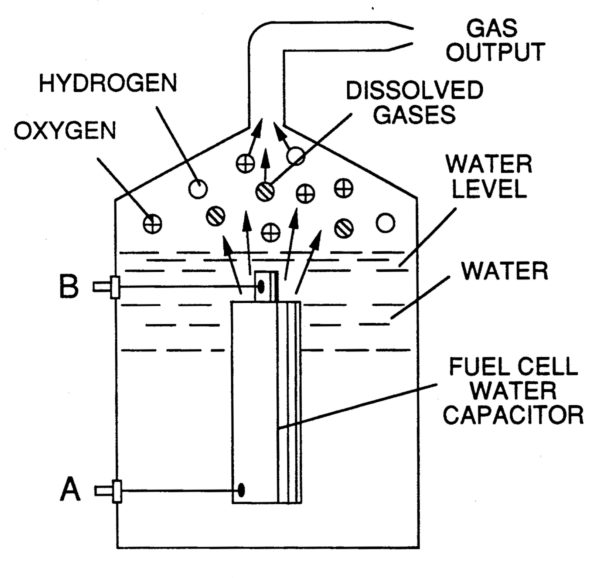
\includegraphics[width=0.5\textwidth]{figures/wfccapacitor}
  \caption{Represantación de la celda en forma de capacitor de Stanley Meyer.}
  \label{fig:wfcc}
\end{figure}


\subsection{Yull Brown} 
A Yull Brown se le otorga el descubirmiento de un mezcla de gas hidrógeno y oxigeno, que al combustionarlo en propociones específicas, produce un gas de caraterísticas diferentes a las del hidrogeno. En su patente~\cite{brown1977welding} Brown hace referencia una forma de soldar al arco~\cite{wiki:arco} utilizando hidrógeno y oxygeno, en donde explica como estos gases son generados. Su aplicación se basa en la aprecición de que existe considerable energía asociada con la disociocion molecular de oxygeno en oxígeno atomico pasando este gas a taves de un acrco, y que esta energía puede ser utilizada para generar temperaturas incluso mayores a las generadas con soldadura de hidrógeno atóimico~\cite{wiki:hidro}. Anteriormente a este invento no era posible pensar en pasar una mezcla de hidrogeno y oxigeno por el arco debido a la naturaleza altamente explosiva e inflamable de los gases, además existe problemas asociados al gas oaxidrogeno en la soldadura debido a que el hidrogeno es absorbido por la mayoria de los metales. Por ejemplo, cuando se solda acero, se debe tener cuidado en asegurar que no existe exceso de hidrogeno porque la abosircion de este provoca que peirda fuerza y fragilidad. Por otro lado, un excedo de oxigeno podría quemar el metal, por lo tanto es imporatante que una mezcla de oxigdrogeno sea ajustada para una flama neutral , es decir, no mucho hidrogeno y no mucho oxigeno. En la practica es dificil ajustar tal mezcla, la solución que se plantea es que las celdas electrolíticas realizan la producción de forma estequimetrica que pasada por el acrco produce una flama neutral~\cite{brown1977welding}.

\subsubsection{Electrolisis}
En su m\'etodo~\cite{brown1977welding} propone una electrólisis en una celda electrolítica~\cite{wiki:electrocell} sin diafragma, que normalmente es utilizado para separa los gases producidos, y dejar que el hidrogeno y el oxigeno se mezclen libremente a una forma estequiometrica que genera una flama neutral. en la patente se especifica ciertas condiciones que debe tener el aparto para la producción de hidrogeno y oxygeno para un mejor producción, estas son enumeradas y muy similares a las de una celda alkalina convencional~\cite{zeng2010recent}.
 
\subsubsection{Genrador de señales}

\subsection{Tay-Hee Han US4427512~\cite{han1984water}}





%\paragraph{George Wiseman}
%% Usos de la electrolisis convecional en la industria y tipos de electrolizadores
%% Usos de la electrólisis no convecional y producto

%\subsection{Modelo Electroquimico de la celda de electrolisis}

%\subsubsection{Resultados}


\subsection{La nueva propuesta}

De que se trata , que es lo diferente

\subsubsection{Fundamento teórico o experimental o esoterico}
Explicación de funcionamiento
mmas tecnico con ecuencaciones y eficiencias esperadas, diagramas

\subsubsection{Eficiencia Electrónica}
\subsubsection{Eficiencia Química}

\paragraph{Modos vibracionales}


\section{Desarrollo}

\subsection{Requerimientos}

Igualar la energía de un capacitor a la energía libre de gibss

\subsection{Diseño de circuito}

\subsubsection{Simulacion}


\subsubsection{Determinar parametros de funcionamiento electrico}
Un dielectrico debilita el campo eléctrico entre placas de un condesador porque sus moléculas producen un campo eléctrico adicional de sentido opuesto al campo externo producido por las placas. Este campo eléctrico se debe a los momentos dipolares eléctricos de las moleculas del dieléctrico~\cite{tipler2005fisica}.

\subsection{Componentes}

\subsection{Diseño Experimento}

%%

\newpage
\bibliographystyle{plain}

\bibliography{Bibliography}{}

%\begin{thebibliography}{99} 
%\bibitem {farad1} J. O. Bockris and T. N. Veziroglu, Int J Hydrogen Energy, 32 (2007) 1605.
%\bibitem{farad2} M. Philippe, H. Jérôme, B. Sebastien and P. Gérard, Electrochim. Acta, 51 (2005) 1140.
%\bibitem{electroview} Kaveh Mazloomi, Nasri b. Sulaiman and Hossein Moayedi. An Investigation into the Electrical Impedance of Water Electrolysis Cells – With a View to Saving Energy. 1 April 2012.
%\bibitem{dublin} Simple Explanation of Meyer Fuel Cell Technology - Dublin Institute of Technology - Industrial Liason Office. year ??
%\bibitem{h2vol} Stensvold, Tore (26 January 2016). «Coca-Cola-oppskrift» kan gjøre hydrogen til nytt norsk industrieventyr. Teknisk Ukeblad.
%%\bibitem{eff}Werner Zittel; Reinhold Wurster (8 July 1996). "Chapter 3: Production of Hydrogen. Part 4: Production from electricity by means of electrolysis". HyWeb: Knowledge – Hydrogen in the Energy Sector. Ludwig-Bölkow-Systemtechnik GmbH. Archived from the original on 7 February 2007.
%\bibitem{wfzero} Water Electrolyzers and the Zero-Point Energy. M. B. King. Space, Propulsion \& Energy Sciences International Forum - 2011.
%\bibitem{alka} Recent progress in alkaline water electrolysis for hydrogen production and applications. Kai Zeng, Dongke Zhang. 2009
%\bibitem{h2owiki} Geometría molecular angular. Wikipedia - La enciclopedia libre. \url{https://es.wikipedia.org/wiki/Geometr%C3%ADa_molecular_angular}
%\bibitem{andrija} Method and Apparatus for Splitting Water Molecules. Andrija Puharich. US Patent 4,394,230 Jul.19, 1983.
%\end{thebibliography} 

\end{document}

